\sectionframe{The Halved Model}
\section{Halved Model}

\begin{frame}{Lifting the Model}
	\vspace{-1em}
	\begin{columns}
		\begin{column}{.4 \textwidth}
			\begin{figure}
				\includegraphics[width=\textwidth]{63_MinimalRepr_Adding_Halved/Cob_Vis_s/Manual/result.png}
			\end{figure}
		\end{column}
		\begin{column}{.5 \textwidth}
			\pause
			\begin{itemize}
				\item Lift the model from $[0, 1)$ to $\mathbb{R}$ \pause
				\item The lifted model repeats every $1$ step \pause
				\item But it even repeats every $\frac{1}{2}$ step because of the built-in symmetry \pause
				\item Drop the model to $[0, \frac{1}{2})$ \pause
			\end{itemize}
			\begin{align*}
				x    & \mapsto g(x) \mod \frac{1}{2}                                            \\
				g(x) & = \begin{cases}
					         l(x) = a_L \cdot x^2 + b_L \cdot x + c_L & \text{ if } x < \frac{1}{4} \\
					         r(x) = b_R \cdot x + c_R                 & \text{ else}
				         \end{cases}
			\end{align*}
		\end{column}
	\end{columns}
\end{frame}

%\begin{frame}{Period-adding in Theory}
%	\begin{columns}
%		\begin{column}{.4 \textwidth}
%			\todo{Pic of halved model function}
%			\todo{Pic of two increasing branches of circle map}
%		\end{column}
%		\begin{column}{.6 \textwidth}
%			\begin{itemize}
%				\item Two increasing branches
%				\item Period-adding proven for non-smooth circle maps with two increasing branches
%			\end{itemize}
%			\todo{reference}
%		\end{column}
%	\end{columns}
%\end{frame}

\begin{frame}{Period-adding in the Halved Model}
	\vspace{-1em}
	\begin{figure}
		\only<1>{
			\includegraphics[width=.4 \textwidth]{63_MinimalRepr_Adding_Halved/1D_Period_larger_adding/Manual/result.png}
			\qquad
			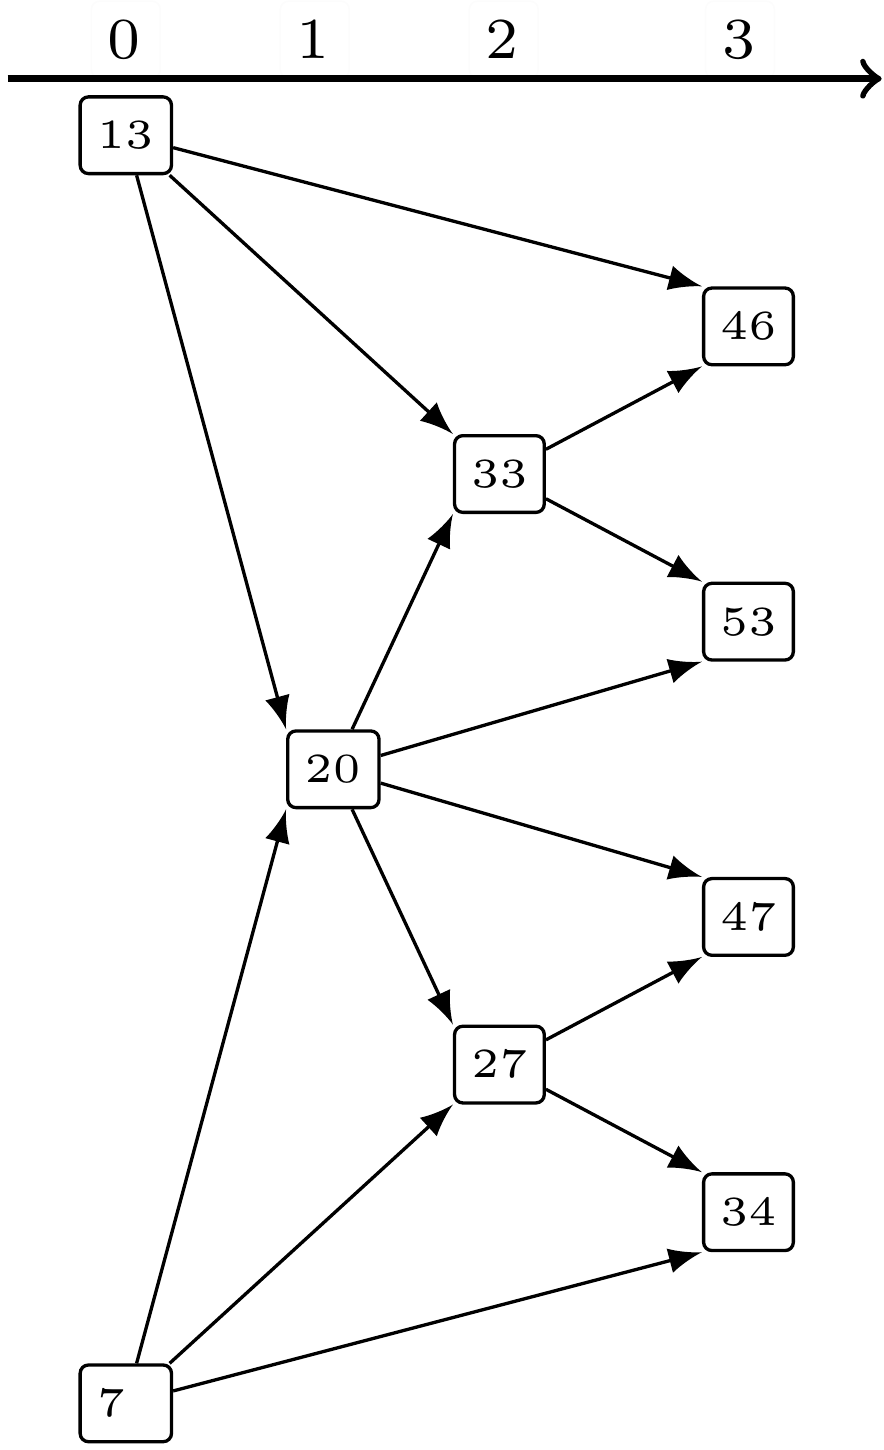
\includegraphics[width=.25 \textwidth]{../../Report/Figures/FareyTrees/Minrep_Adding_larger_Halved_Period_3/adding.pdf}
		}
		\only<2>{
			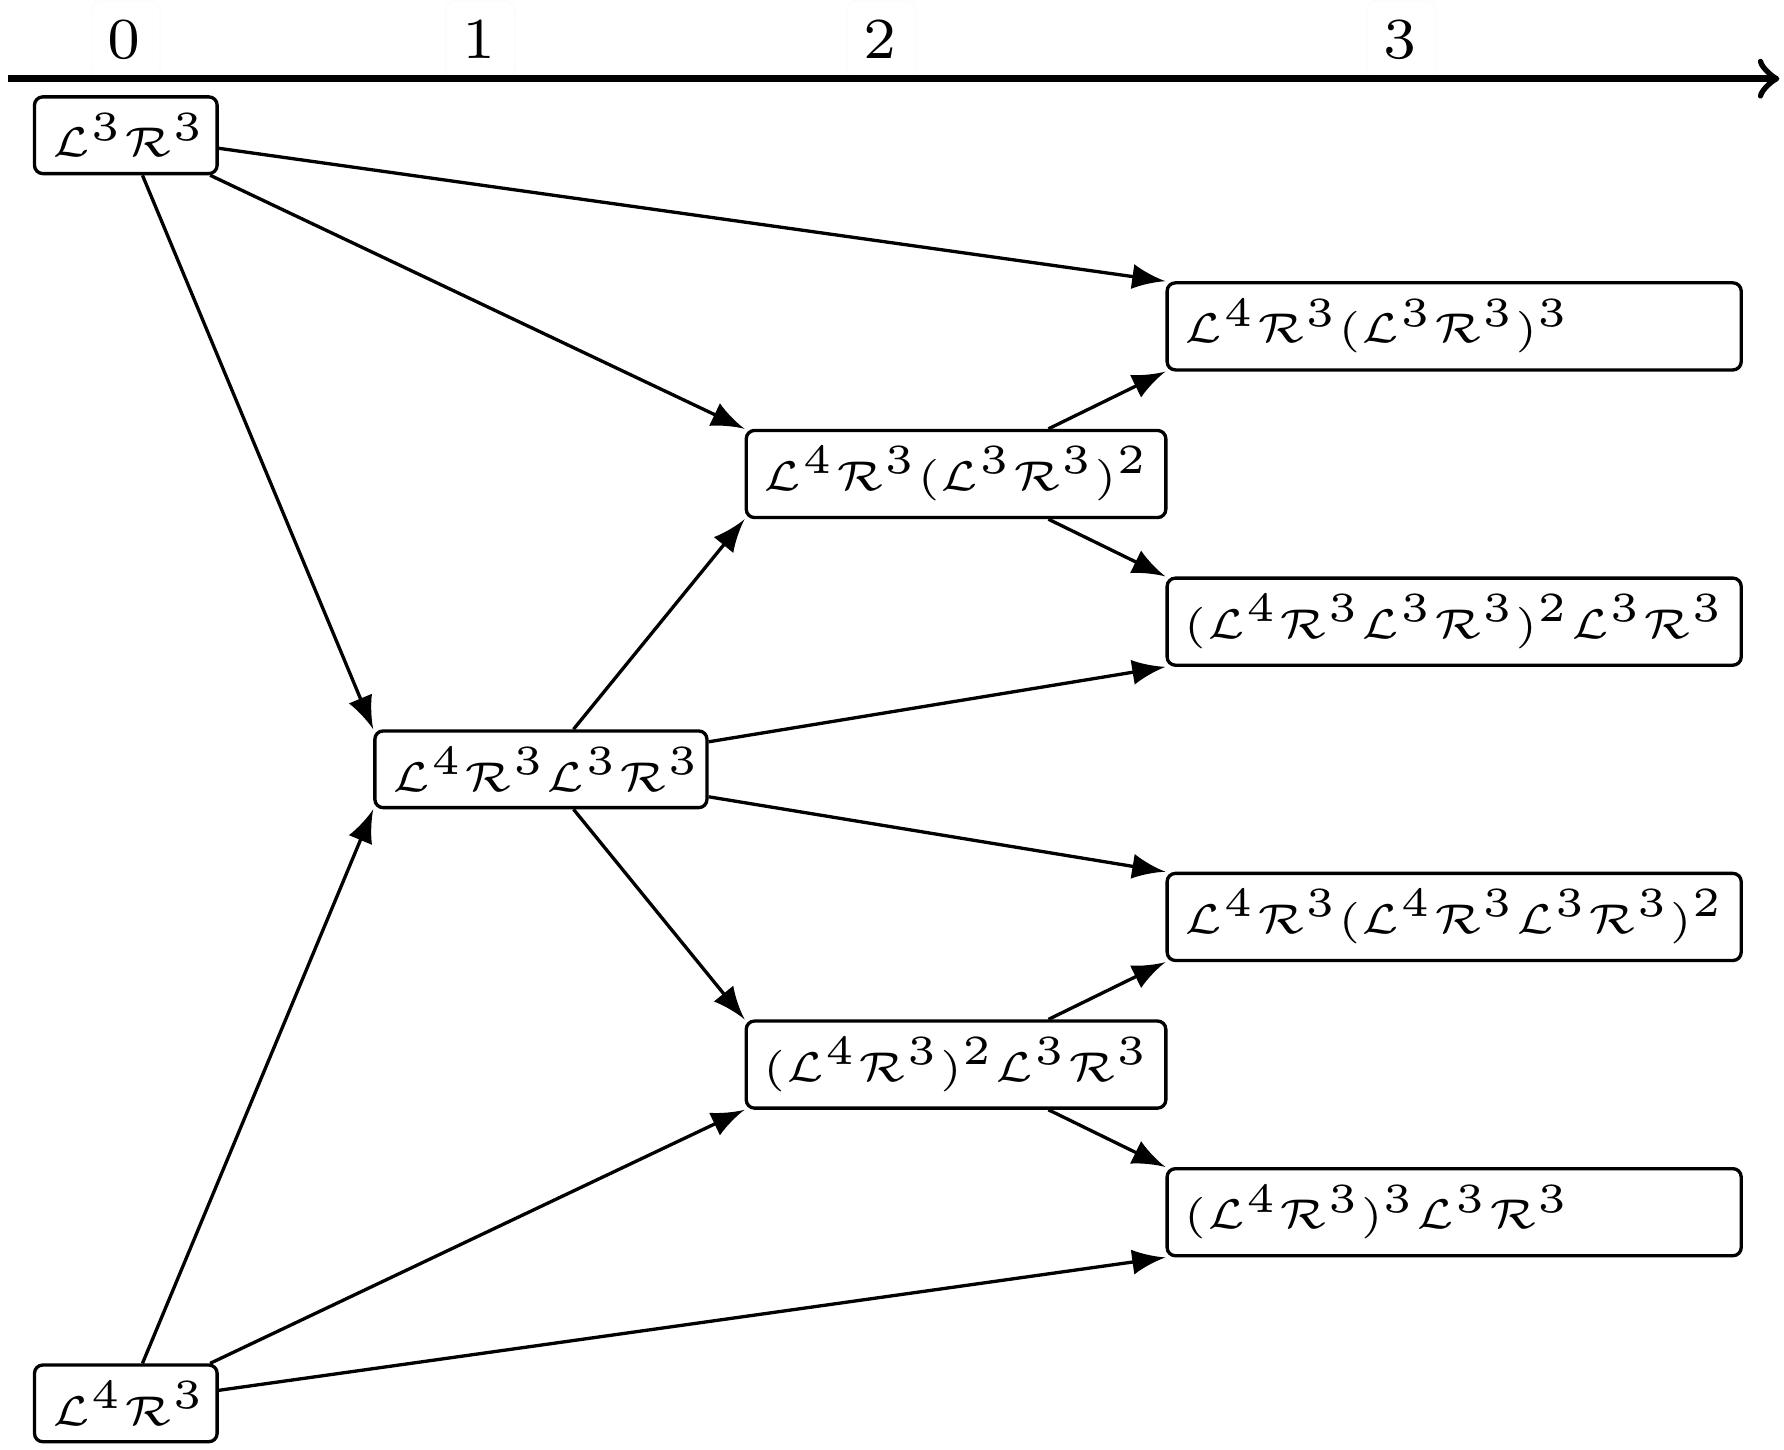
\includegraphics[width=.6 \textwidth]{../../Report/Figures/FareyTrees/Minrep_Adding_larger_Halved_3/adding.pdf}
		}
	\end{figure}
\end{frame}

\begin{frame}{Period-adding in the Halved Model}
	\vspace{-1em}
	\begin{columns}
		\begin{column}{.7 \textwidth}
			\begin{itemize}
				\item Periods add up!
				\item Symbolic sequences concatenate!
			\end{itemize}
			\pause
			\begin{center}
				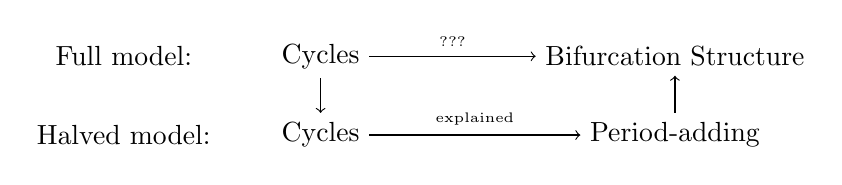
\begin{tikzpicture}
					\node (FM) at (0, 1) {Full model:};
					\node (FC) at (2.5, 1) {Cycles};
					\node (FB) at (7, 1) {Bifurcation Structure};

					\node (HM) at (0, 0) {Halved model:};
					\node (HC) at (2.5, 0) {Cycles};
					\node (HA) at (7, 0) {Period-adding};

					\draw[->] (FC) -- (HC);
					\draw[->] (HC) -- (HA) node[midway,above] {\tiny explained};
					\draw[->] (HA) -- (FB);
					\draw[->] (FC) -- (FB) node[midway,above] {\tiny ???};
				\end{tikzpicture}
			\end{center}
			\vspace{1em}
			\pause
			Allegory of the cave (``Höhlengleichnis'') type of situation
		\end{column}
		\begin{column}{.3 \textwidth}
			\vspace{2em}
			\only<3->{
				\begin{figure}
					
\includegraphics[width=\textwidth]{Figs/allegory.jpeg}
				\end{figure}
			}
		\end{column}
	\end{columns}
\end{frame}

\begin{frame}{Some Definitions}
	\vspace{-1em}
	\begin{definition}[Syllables]
		A syllable is a maximal sequence of the same symbol. \\[1em]
		A pair of syllables next to each other is called a 2-syllable.
		A 4-syllable is a quadrupel of syllables next to each other.
	\end{definition}
	\pause
	Example: $\L^4\R^3\L^3\R^3$ has the syllables $\L^4$, $\L^3$, and $\R^3$ twice.
	\vspace{1em}
	\begin{itemize}
		\pause
		\item One rotation in the halved model corresponds to one 2-syllable \pause
		\item One rotation in the full model corresponds to one 4-syllable \pause
		\item One rotation in the full model corresponds to 2 rotations in the halved model
	\end{itemize}
\end{frame}

\begin{frame}{Translating Symbolic Sequences}
	\begin{definition}[Translating 4-syllables]
		The function $t$ translates one 4-syllable from the halved model to one 4-syllable in the full model.
		\begin{align*}
			t: \L^a\R^b\L^c\R^d \mapsto \A^a\B^b\C^c\D^d
		\end{align*}
	\end{definition}

	\pause
	From the ad-hoc method:
	\pause
	\begin{itemize}
		\item We can only translate 4-syllables (2 rotations in the halved model) at a time \pause
		\item Especially: We cannot translate a 2-syllable alone
	\end{itemize}
	\pause
	So if the cycle in the halved model has an odd number of rotations (2-syllables) we need to wrap around once while translating.
\end{frame}

\begin{frame}{The First Consequences}
	\begin{theorem}[Periods and Coexistence in the Full Model]
		An $n$-cycle in the halved model manifests as
		\begin{itemize}
			\item a single $2n$-cycle in the full model if it has an odd number of rotations
			\item 2 coexisting $n$-cycles in the full model if it has an even number of rotations
		\end{itemize}
	\end{theorem}
	\pause
	Examples:
	\begin{itemize}
		\item $\L^4\R^3$ (Period 7) manifests as a single cycle $\A^4\B^3\C^4\D^3$ (Period 14)
		\item $\L^4\R^3\L^3\R^3$ (Period 13) manifests as two cycles
		      \begin{itemize}
			      \item $\A^4\B^3\C^3\D^3$ (Period 13) and
			      \item $\A^3\B^3\C^4\D^3$ (Period 13)
		      \end{itemize}
	\end{itemize}
\end{frame}

\begin{frame}{The First Consequences}
	\vspace{-1em}
	\only<1-3>{
		\begin{theorem}[Coexistence in Child Nodes]
			A node in the Farey-tree is associated
			\begin{itemize}
				\item with a single cycle if
				      \begin{itemize}
					      \item one parent node is associated with 2 coexisting cycles and the other parent node is associated with a single cycle.
				      \end{itemize}
				      \pause
				\item with two coexisting cycles if
				      \begin{itemize}
					      \item both parent nodes are associated with single cycles, or
					      \item both parent nodes are associated with two coexisting cycles each.
				      \end{itemize}
			\end{itemize}
		\end{theorem}
		\pause
		\begin{itemize}
			\item The third case does not appear in our adding structures
			\item We will omit this case in following rules
		\end{itemize}
	}
	\only<4>{
		\begin{figure}
			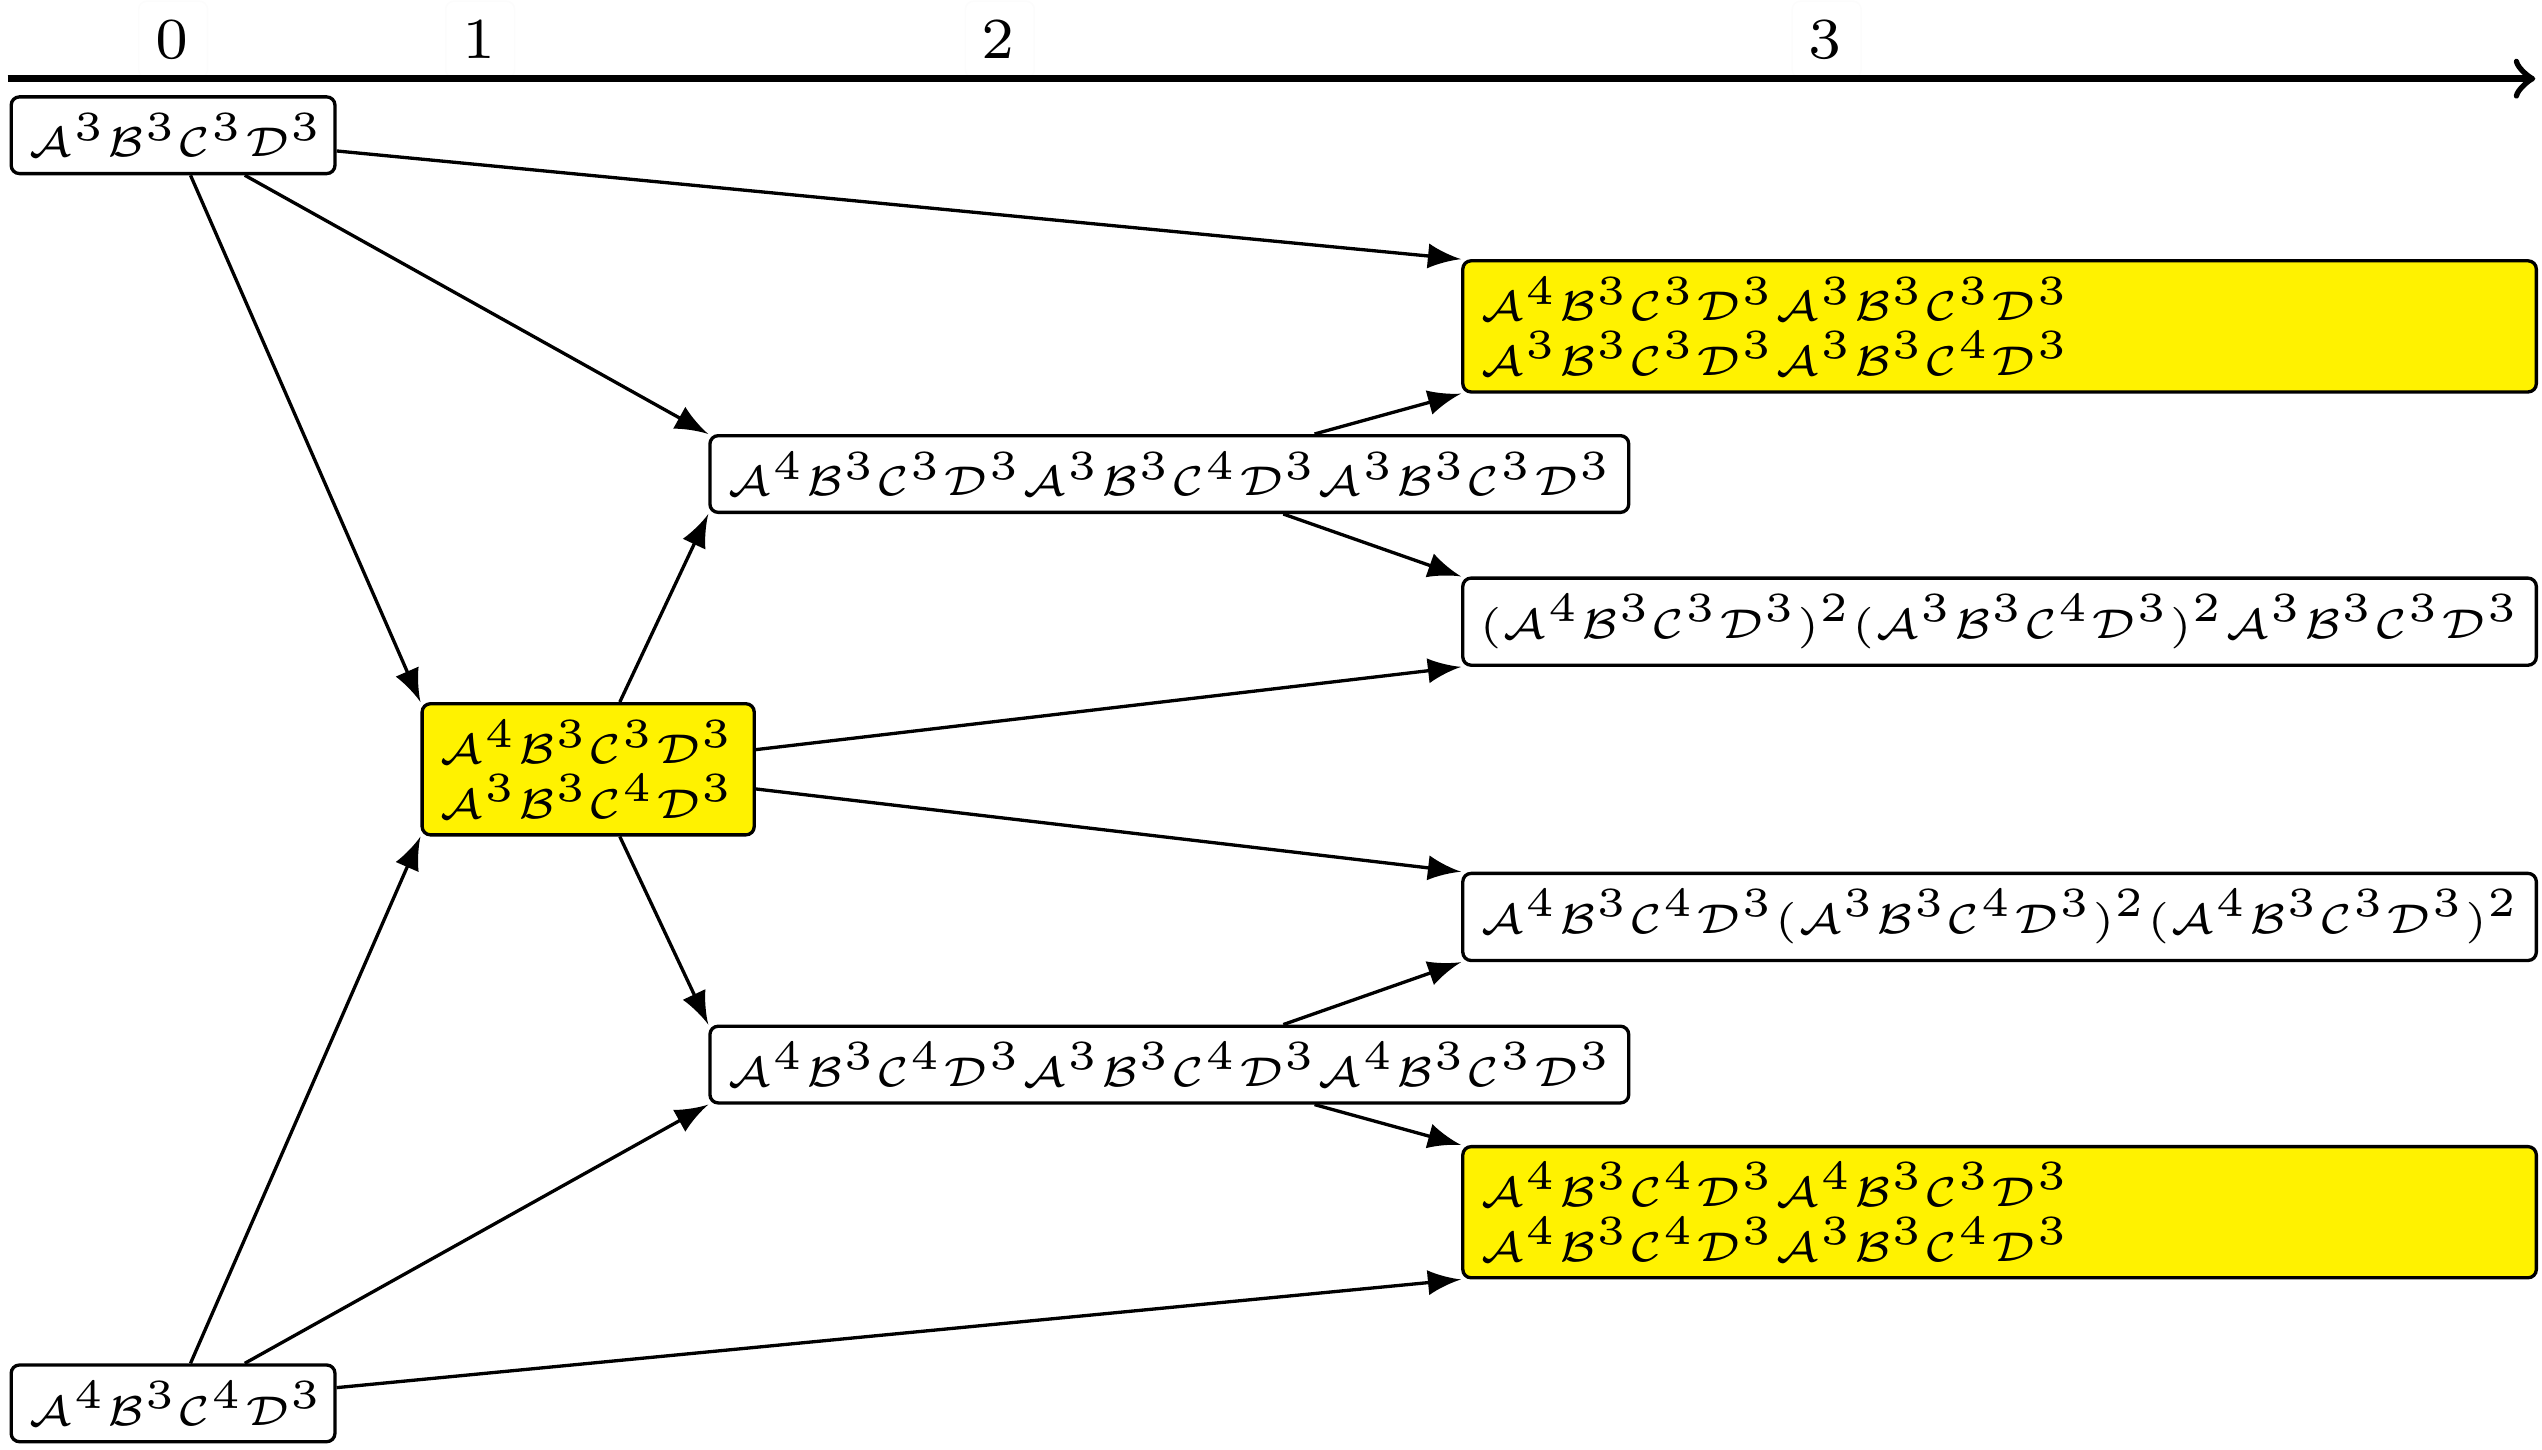
\includegraphics[width=.7 \textwidth]{../../Report/Figures/FareyTrees/Minrep_Adding_larger_Full_3/adding.pdf}
		\end{figure}
	}
\end{frame}

\begin{frame}{``Concatenation'' in the Full Model}
	\vspace{-1em}
	\begin{theorem}[Cycles in Child Nodes of two Nodes with Singular Cycles]
		The cycles $\pi^a$ and $\pi^b$ of a node with two parents with a singular cycle each, $\phi$ and $\psi$ are
		\begin{align*}
			\pi^a = \phi_1 \dots \phi_{\frac{n-1}{2}} \left[\phi_{\frac{n+1}{2}} \mid \psi_{\frac{m+1}{2}}\right] \psi_{\frac{m+3}{2}} \dots \psi_m
		\end{align*}
		and
		\begin{align*}
			\pi^b =  \phi_{\frac{n+3}{2}} \dots \phi_n \psi_1 \dots \psi_{\frac{m-1}{2}} \left[\psi_{\frac{m+1}{2}} \mid \phi_{\frac{n+1}{2}}\right]
		\end{align*}
	\end{theorem}
	\pause
	Example: \vspace{-2em} \begin{align*}
		\phi                    & = \A^4\B^3\C^4\D^3, \psi = \A^3\B^3\C^3\D^3  \\
		\Rightarrow \quad \pi^a & = \A^4\B^3\C^3\D^3, \pi^b = \A^3\B^3\C^4\D^3
	\end{align*}
\end{frame}

\begin{frame}{``Concatenation'' in the Full Model}
	\vspace{-1em}
	\begin{theorem}[Cycles in Child Nodes of Parent Nodes with Different Multiplicity]
		The cycle $\pi$ of a node with one parent with a single cycle $\phi$ and one parent with two coexisting cycles $\psi^a$ and $\psi^b$ is either
		\begin{itemize}
			\item If $\phi$ is associated with the left parent node
			      \begin{align*}
				      \pi = \phi_1 \dots \phi_{\frac{n-1}{2}} \left[\phi_{\frac{n+1}{2}} \mid \psi^b_m\right] \psi^b_1 \dots \psi^b_{m-1} \left[\psi^b_m \mid \phi_{\frac{n+1}{2}}\right] \phi_{\frac{n+3}{2}} \dots \phi_n \psi^a
			      \end{align*}
			\item If $\phi$ is associated with the right parent node
			      \begin{align*}
				      \pi = \psi^a \phi_1 \dots \phi_{\frac{n-1}{2}} \left[\phi_{\frac{n+1}{2}} \mid \psi^b_m\right] \psi^b_1 \dots \psi^b_{m-1} \left[\psi^b_m \mid \phi_{\frac{n+1}{2}}\right] \phi_{\frac{n+3}{2}} \dots \phi_n
			      \end{align*}
		\end{itemize}
	\end{theorem}
\end{frame}

\begin{frame}{Explained Bifurcation Structures}
	\begin{figure}
		\only<1>{
			\includegraphics[width=.4 \textwidth]{62_MinimalRepr_Adding/1D_Period_larger_adding/Manual/result.png}
			\qquad
			\includegraphics[width=.4 \textwidth]{63_MinimalRepr_Adding_Halved/1D_Period_larger_adding/Manual/result.png}
		}
		\only<2>{
			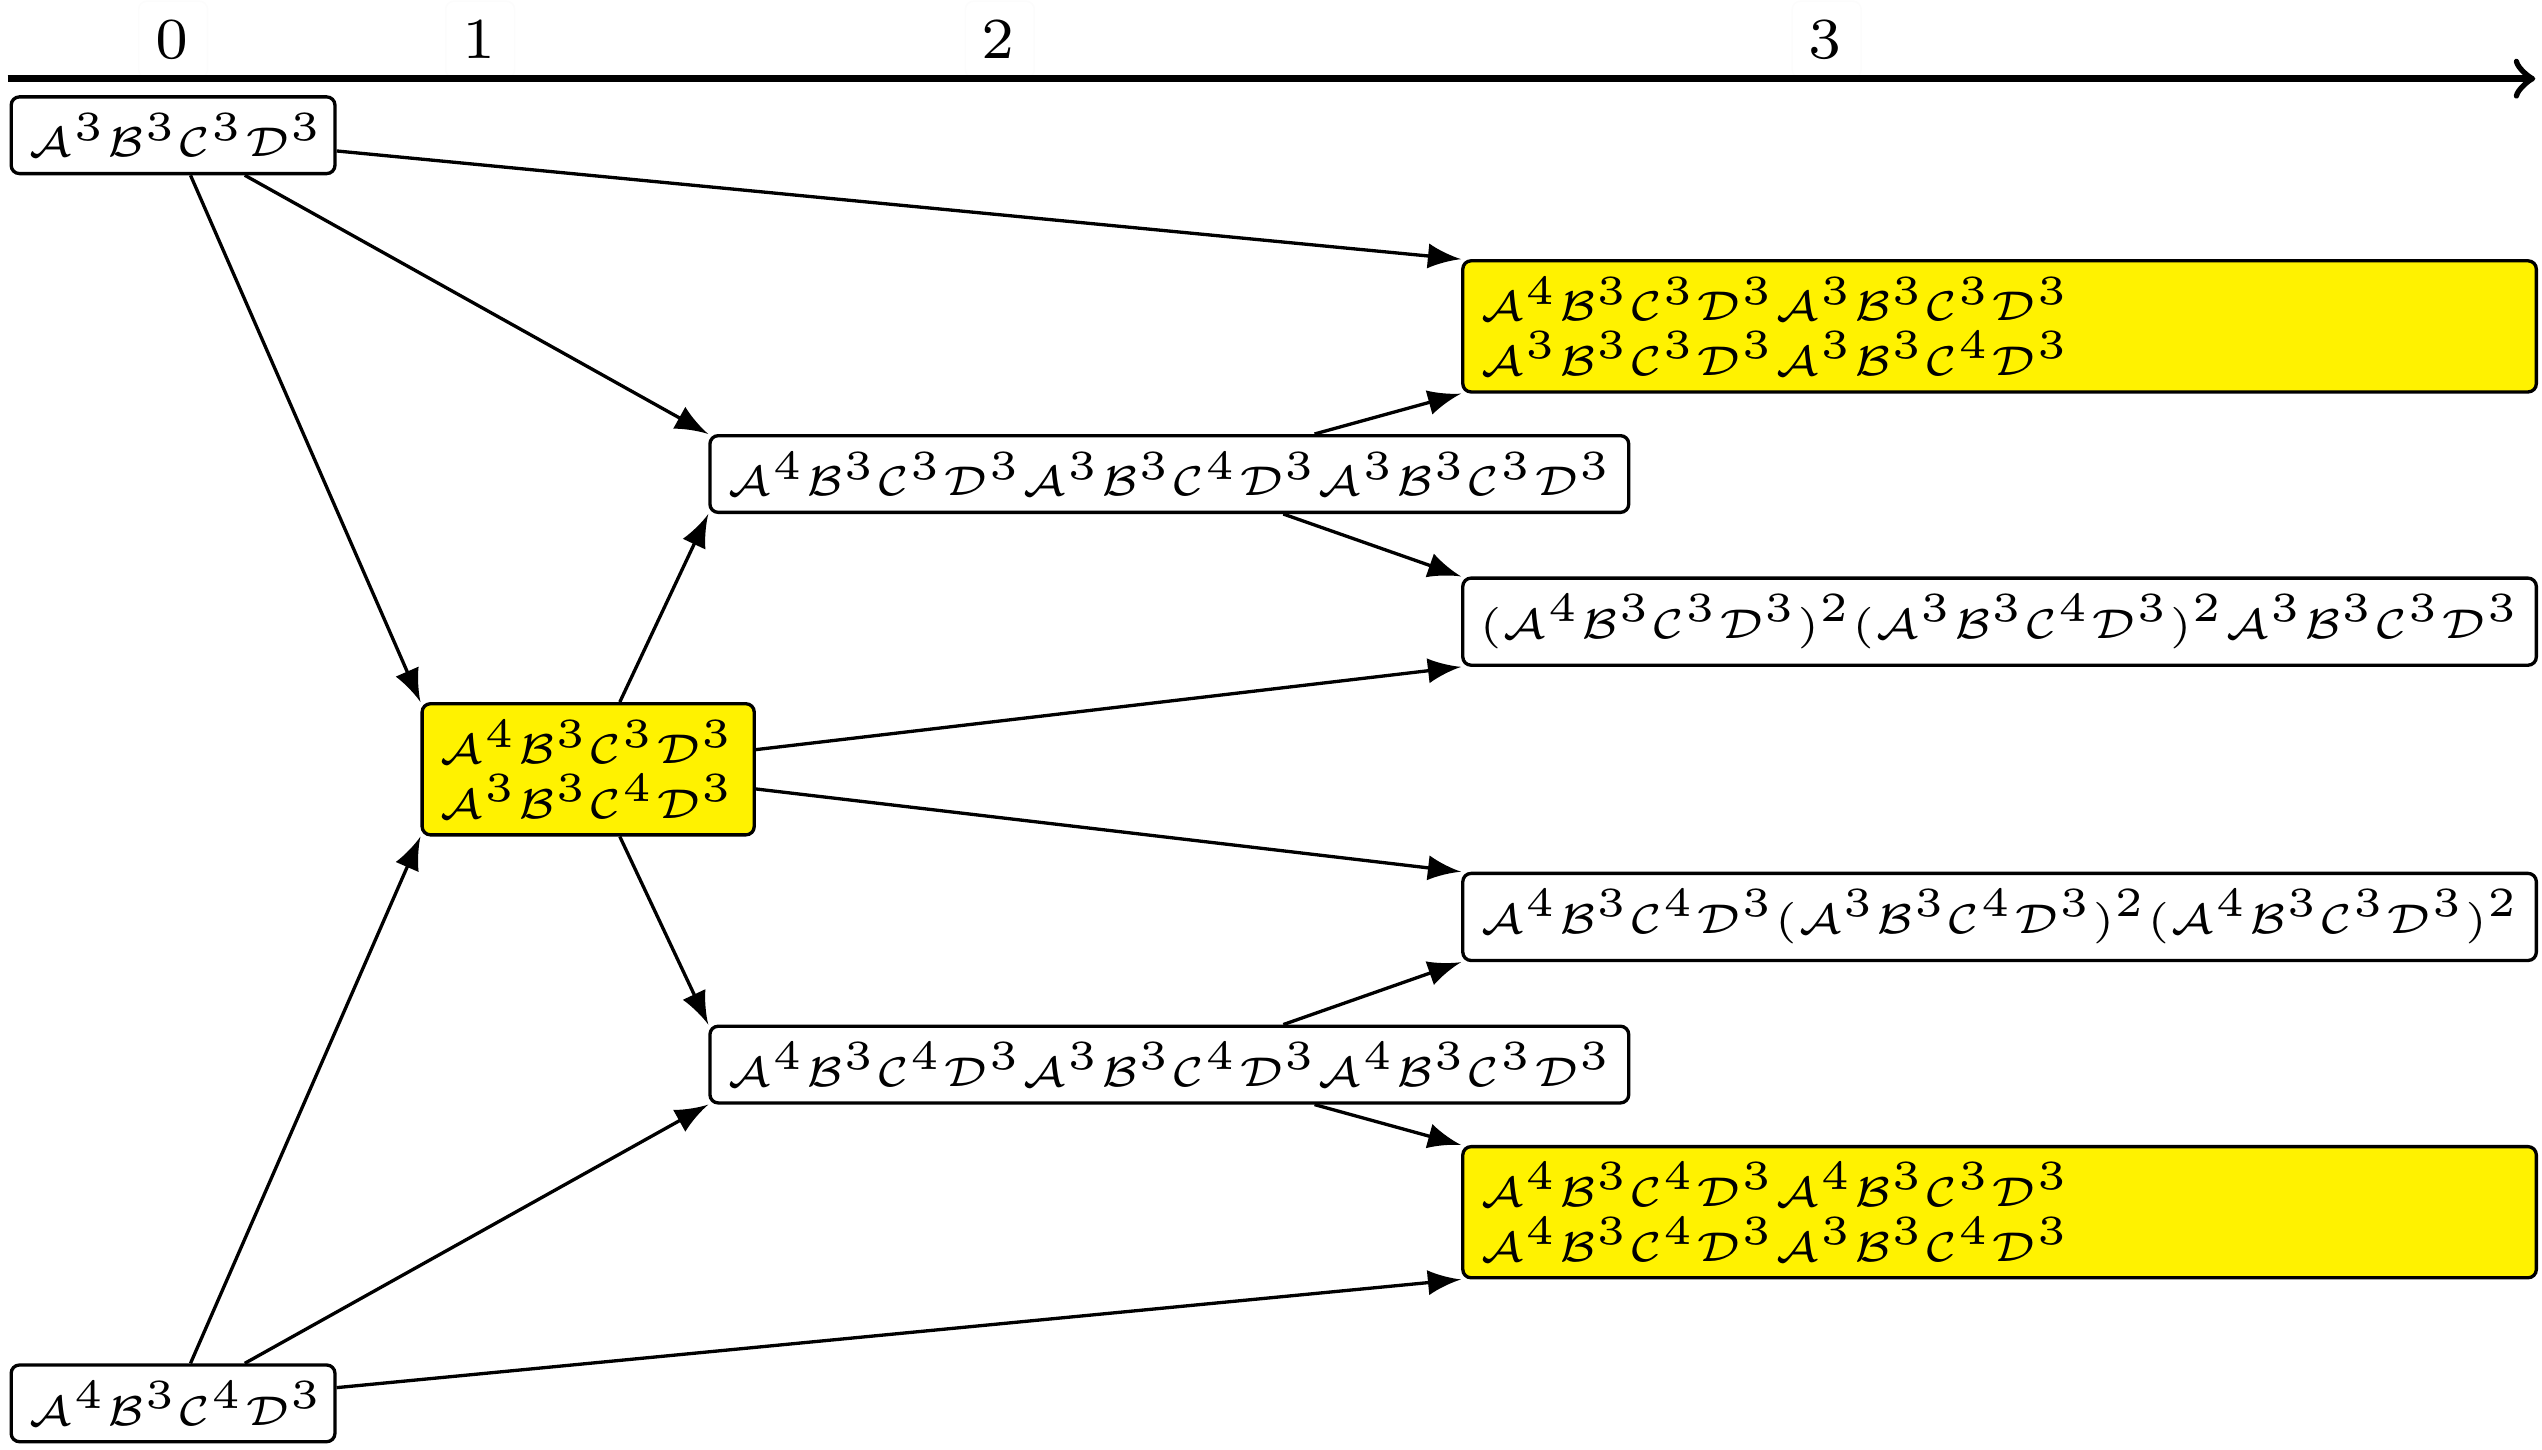
\includegraphics[width=.525 \textwidth]{../../Report/Figures/FareyTrees/Minrep_Adding_larger_Full_3/adding.pdf}
			\qquad
			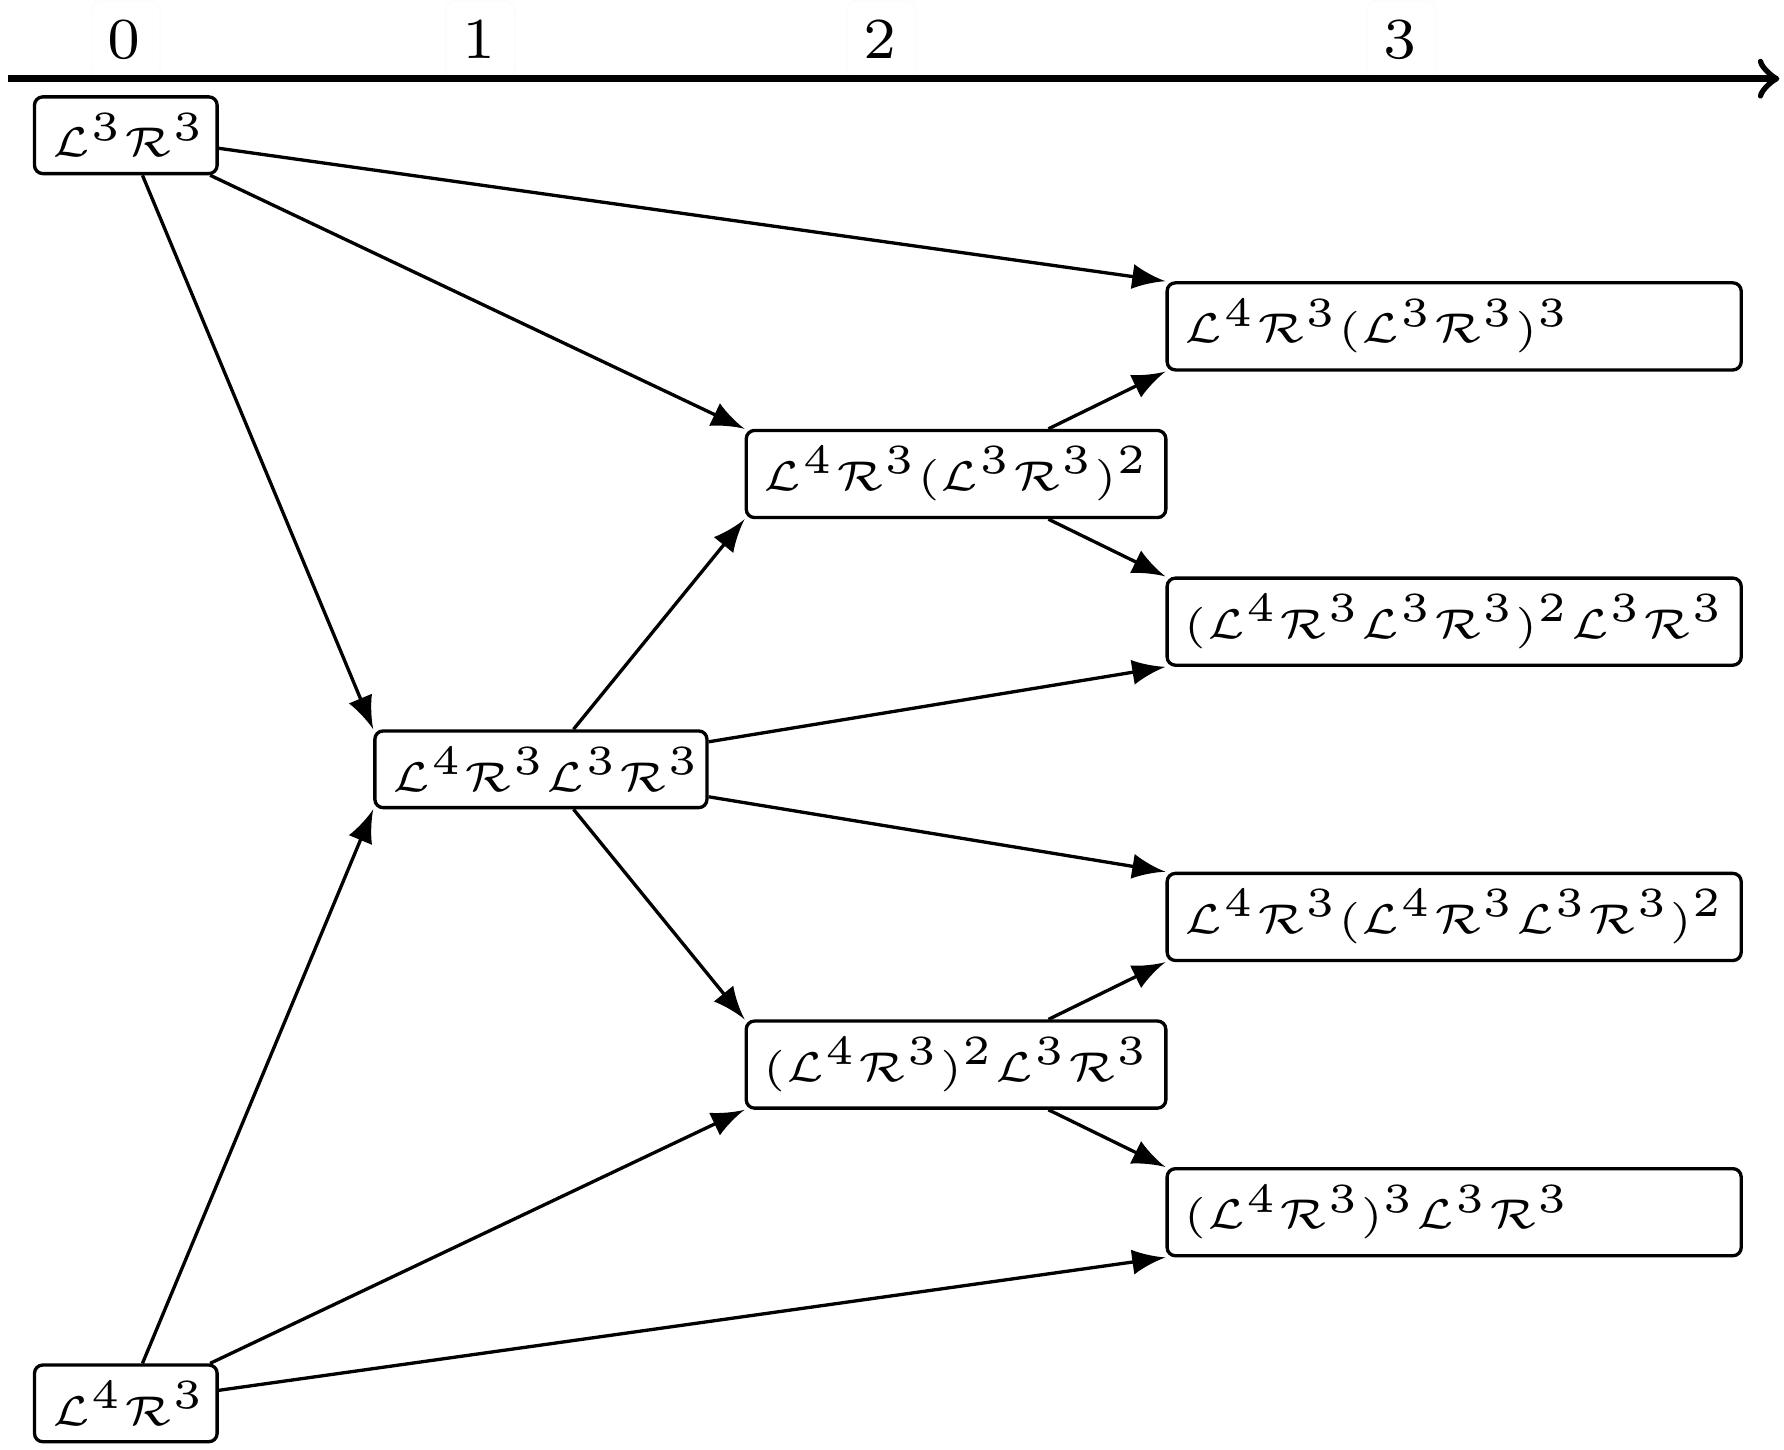
\includegraphics[width=.4 \textwidth]{../../Report/Figures/FareyTrees/Minrep_Adding_larger_Halved_3/adding.pdf}
		}
	\end{figure}
\end{frame}

\begin{frame}{Rotation Numbers}
	\begin{itemize}
		\item Also found rules for rotation numbers
		\item Limited time in this presentation
	\end{itemize}
\end{frame}

%\begin{frame}{Rotation Tuples}
%	\vspace{-1em}
%    \begin{theorem}[Rotation Tuples in Child Nodes of Two Nodes with Singular Cycles]
%		The cycles $\pi^a$ and $\pi^b$ of a node with two parents with a singular cycle each, $\phi$ and $\psi$ have the rotation tuples
%		\begin{columns}
%			\begin{column}{.7 \textwidth}
%				\begin{align*}
%					\rho_\A(\pi^a) & = \frac{|\phi_1 \dots \phi_{\frac{n+1}{2}}|_\A + |\psi_{\frac{m+3}{2}} \dots \psi_m|_\A}{|\pi|} \\
%					\rho_\B(\pi^a) & = \frac{|\phi_1 \dots \phi_{\frac{n+1}{2}}|_\B + |\psi_{\frac{m+3}{2}} \dots \psi_m|_\B}{|\pi|} \\
%					\rho_\C(\pi^a) & = \frac{|\phi_1 \dots \phi_{\frac{n-1}{2}}|_\C + |\psi_{\frac{m+1}{2}} \dots \psi_m|_\C}{|\pi|} \\
%					               & \vdots
%				\end{align*}
%			\end{column}
%			\begin{column}{.3 \textwidth}
%				\begin{align*}
%					|\pi| & = |\pi^a| = |\pi^b|         \\
%					      & = \frac{|\phi| + |\psi|}{2}
%				\end{align*}
%			\end{column}
%		\end{columns}
%	\end{theorem}
%\end{frame}

%\begin{frame}{Rotation Tuples}[Rotation Tuples in Child Nodes of Parent Nodes with Different Multiplicity]
%	\begin{theorem}
%		The cycle $\pi$ of a node with one parent with a single cycle $\phi$ and one parent with two coexisting cycles $\psi^a$ and $\psi^b$ has the rotation tuple
%		\begin{align*}
%			\rho(\pi) = \rho(\phi) \oplus \rho(\psi^a) \oplus \rho(\psi^b)
%		\end{align*}
%		Where the farey-addition of tuples is element-wise.
%	\end{theorem}
%\end{frame}
